\let\negmedspace\undefined
\let\negthickspace\undefined
\documentclass[journal]{IEEEtran}
\usepackage[a5paper, margin=10mm, onecolumn]{geometry}
\usepackage{lmodern} % Ensure lmodern is loaded for pdflatex
\usepackage{tfrupee} % Include tfrupee package

\setlength{\headheight}{1cm} % Set the height of the header box
\setlength{\headsep}{0mm}     % Set the distance between the header box and the top of the text

\usepackage{gvv-book}
\usepackage{gvv}
\usepackage{cite}
\usepackage{amsmath,amssymb,amsfonts,amsthm}
\usepackage{algorithmic}
\usepackage{graphicx}
\graphicspath{{./figs/}}
\usepackage{textcomp}
\usepackage{xcolor}
\usepackage{txfonts}
\usepackage{listings}
\usepackage{enumitem}
\usepackage{mathtools}
\usepackage{gensymb}
\usepackage{comment}
\usepackage[breaklinks=true]{hyperref}
\usepackage{tkz-euclide} 
\usepackage{listings}
\usepackage{gvv}                                        
\def\inputGnumericTable{}                                 
\usepackage[latin1]{inputenc}                                
\usepackage{color}                                            
\usepackage{array}                                            
\usepackage{longtable}                                       
\usepackage{calc}                                             
\usepackage{multirow}                                         
\usepackage{hhline}                                           
\usepackage{ifthen}                                           
\usepackage{lscape}
\usepackage{circuitikz}
\tikzstyle{block} = [rectangle, draw, fill=blue!20, 
text width=4em, text centered, rounded corners, minimum height=3em]
\tikzstyle{sum} = [draw, fill=blue!10, circle, minimum size=1cm, node distance=1.5cm]
\tikzstyle{input} = [coordinate]
\tikzstyle{output} = [coordinate]
\begin{document}
\bibliographystyle{IEEEtran}
\vspace{3cm}
\title{2.10.78}
\author{EE25BTECH11050-Hema Havil}
	\maketitle
	% \newpage
	% \bigskip
	{\let\newpage\relax\maketitle}
	
	\renewcommand{\thefigure}{\theenumi}
	\renewcommand{\thetable}{\theenumi}
	\setlength{\intextsep}{12pt} % Space between text and floats
	
	\numberwithin{equation}{enumi}
	\numberwithin{figure}{enumi}
	\renewcommand{\thetable}{\theenumi}
	
	\textbf{Question}:\\
    
         The point (4, 1) undergoes the following three transformations successively.
         \begin{enumerate}[label=(\alph*)]
             \item Reflection about the line $y = x$.
             \item Translation through a distance 2 units along the positive direction of x-axis.
             \item Rotation through an angle $\frac{\pi}{4}$ about the origin in the counter clockwise direction.
         \end{enumerate}
         Then the final position of the point is given by the coordinates.
         \begin{multicols}{4}
             \begin{enumerate}[label=(\alph*)]
                \item $\brak{\frac{1}{\sqrt{2}},\frac{7}{\sqrt{2}}}$
                \item $\brak{-\sqrt{2},7\sqrt{2}}$
                \item $\brak{\sqrt{2},7\sqrt{2}}$
                \item $\brak{-\frac{1}{\sqrt{2}},\frac{7}{\sqrt{2}}}$
             \end{enumerate}
         \end{multicols}
         
         \solution \\
         Let the given point be P=(4,1) and vector be $\vec{P}=\myvec{4\\1}$,
         \begin{enumerate}[label=(\alph*)]
             \item Reflection matrix for $y=x$ is,
             \begin{align}
                 \vec{M}=\myvec{0\;1\\1\;0}
             \end{align}
             then the reflection of P about $y=x$ is,
             \begin{align}
                 \vec{P_1}=\vec{M}\vec{P}
             \end{align}
             \begin{align}
                 \vec{P_1}=\myvec{0\;1\\1\;0}\myvec{4\\1}
             \end{align}
             \begin{align}
                 \vec{P_1}=\myvec{1\\4}
             \end{align}
             \item Translate point $P_1=(1,4)$, 2 units along the positive direction of x axis,
             \begin{align}
                 \vec{P_2} = \vec{P_1} + \vec{X}
             \end{align}
             where X=(2,0)
             \begin{align}
                 \vec{P_2} = \myvec{1\\4}+\myvec{2\\0}
             \end{align}
             \begin{align}
                 \vec{P_2} = \myvec{3\\4}
             \end{align}
             \item Rotation matrix is given as,
             \begin{align}
                 \vec{R}=\myvec{cos\theta\;-sin\theta\\sin\theta\;\;\;\;\;cos\theta}
             \end{align}
             Rotation of $P_2$ by an angle $\frac{\pi}{4}$ about the origin in the counter clockwise direction, substitute $\frac{\pi}{4}$ in R
             \begin{align}
                 \vec{P_3}=\vec{R}\vec{P_2}
             \end{align}
             \begin{align}
                 \vec{P_3}=\myvec{\frac{1}{\sqrt{2}}\;-\frac{1}{\sqrt{2}}\\\frac{1}{\sqrt{2}}\;\;\;\;\frac{1}{\sqrt{2}}}\myvec{3\\4}
             \end{align}
             \begin{align}
                 \vec{P_3}=\myvec{-\frac{1}{\sqrt{2}}\\\frac{7}{\sqrt{2}}}
             \end{align}
             Therefore the final position of the point is $P_3=(-\frac{1}{\sqrt{2}},\frac{7}{\sqrt{2}})$, option (d) is correct
             \end{enumerate}
             \begin{figure}[h]
                 \centering
                 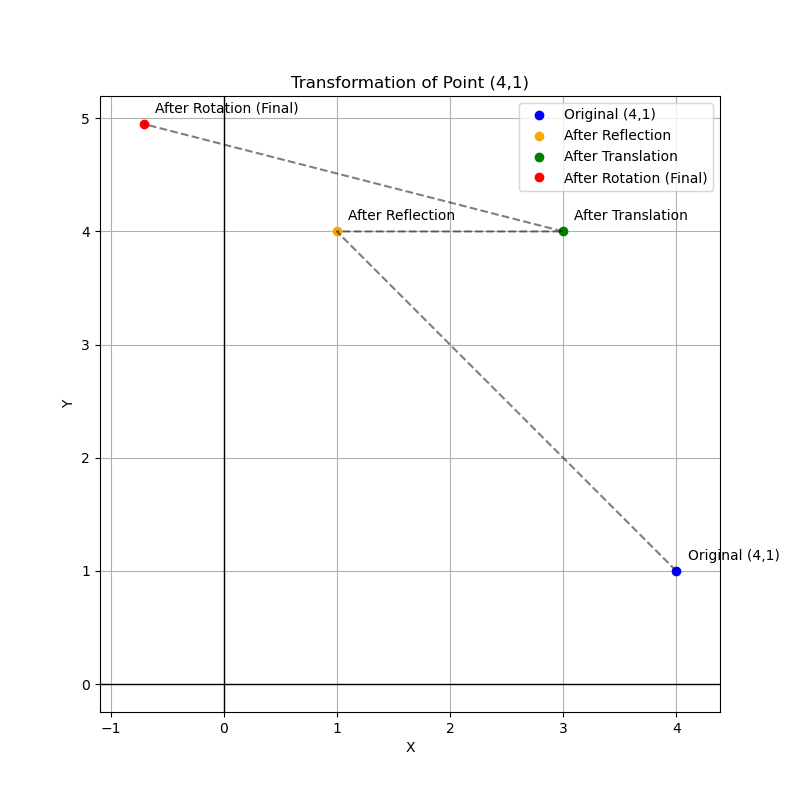
\includegraphics[width=0.9\columnwidth]{figs/fig1.png}
                 \caption{Plot for the above Transformations}
                 \label{fig1}
             \end{figure}
         
\end{document}
